\documentclass[
  man,
  floatsintext,
  colorlinks=true,linkcolor=blue,citecolor=blue,urlcolor=blue,biblatex]{apa7}

% TODO: Add custom LaTeX header directives here
\makeatletter
\renewcommand{\paragraph}{\@startsection{paragraph}{4}{\parindent}%
	{0\baselineskip \@plus 0.2ex \@minus 0.2ex}%
	{-.5em}%
	{\normalfont\normalsize\bfseries\typesectitle}}

\renewcommand{\subparagraph}[1]{\@startsection{subparagraph}{5}{0.5em}%
	{0\baselineskip \@plus 0.2ex \@minus 0.2ex}%
	{-\z@\relax}%
	{\normalfont\normalsize\bfseries\itshape\hspace{\parindent}{#1}\textit{\addperi}}{\relax}}
\makeatother
\usepackage{fontspec}
\usepackage{multirow}
\usepackage{multicol}
\usepackage{colortbl}
\usepackage{hhline}
\newlength\Oldarrayrulewidth
\newlength\Oldtabcolsep
\usepackage{longtable}
\usepackage{array}
\usepackage{hyperref}
\usepackage{float}
\usepackage{wrapfig}\makeatletter\makeatother\makeatletter\makeatother\makeatletter\@ifpackageloaded{caption}{}{\usepackage{caption}}\AtBeginDocument{%
\ifdefined\contentsname
  \renewcommand*\contentsname{Table of contents}
\else
  \newcommand\contentsname{Table of contents}
\fi
\ifdefined\listfigurename
  \renewcommand*\listfigurename{List of Figures}
\else
  \newcommand\listfigurename{List of Figures}
\fi
\ifdefined\listtablename
  \renewcommand*\listtablename{List of Tables}
\else
  \newcommand\listtablename{List of Tables}
\fi
\ifdefined\figurename
  \renewcommand*\figurename{Figure}
\else
  \newcommand\figurename{Figure}
\fi
\ifdefined\tablename
  \renewcommand*\tablename{Table}
\else
  \newcommand\tablename{Table}
\fi
}\@ifpackageloaded{float}{}{\usepackage{float}}
\floatstyle{ruled}
\@ifundefined{c@chapter}{\newfloat{codelisting}{h}{lop}}{\newfloat{codelisting}{h}{lop}[chapter]}
\floatname{codelisting}{Listing}\newcommand*\listoflistings{\listof{codelisting}{List of Listings}}\makeatother\makeatletter\@ifpackageloaded{caption}{}{\usepackage{caption}}
\@ifpackageloaded{subcaption}{}{\usepackage{subcaption}}\makeatother\makeatletter\@ifpackageloaded{tcolorbox}{}{\usepackage[skins,breakable]{tcolorbox}}\makeatother\makeatletter\@ifundefined{shadecolor}{\definecolor{shadecolor}{rgb}{.97, .97, .97}}\makeatother\makeatletter\makeatother



\usepackage[style=apa,backend=biber]{biblatex}
\addbibresource{bibliography.bib}

\newlength{\cslhangindent}
\setlength{\cslhangindent}{1.5em}
\newlength{\csllabelwidth}
\setlength{\csllabelwidth}{3em}
\newlength{\cslentryspacingunit} % times entry-spacing
\setlength{\cslentryspacingunit}{\parskip}
\newenvironment{CSLReferences}[2] % #1 hanging-ident, #2 entry spacing
 {% don't indent paragraphs
  \setlength{\parindent}{0pt}
  % turn on hanging indent if param 1 is 1
  \ifodd #1
  \let\oldpar\par
  \def\par{\hangindent=\cslhangindent\oldpar}
  \fi
  % set entry spacing
  \setlength{\parskip}{#2\cslentryspacingunit}
 }%
 {}
\usepackage{calc}
\newcommand{\CSLBlock}[1]{#1\hfill\break}
\newcommand{\CSLLeftMargin}[1]{\parbox[t]{\csllabelwidth}{#1}}
\newcommand{\CSLRightInline}[1]{\parbox[t]{\linewidth - \csllabelwidth}{#1}\break}
\newcommand{\CSLIndent}[1]{\hspace{\cslhangindent}#1}

\title{Using Quarto to Generate MS Word Documents in APA Style (7th
Edition)}
\shorttitle{Template for the APAquarto Format}




\authorsnames[{1,2},{1},{3,4},{5}]{
Ana Fulana,Blanca Zutana,Carina Mengana,Dolorita Perengana
}

\authorsaffiliations{
{Department of Psychology, Ana and Blanca's University},{Ana's Secondary
Affiliation},{Carina's Primary Affiliation},{Carina's Secondary
Affiliation},{Buffalo, NY }}

\date{}
\abstract{This document is a template demonstrating the apaquarto
format.}
\addbibresource{bibliography.bib}

\keywords{keyword1, keyword2, keyword3}

\authornote{\par{\addORCIDlink{Ana
Fulana}{0000-0000-0000-0000}}\par{\addORCIDlink{Carina
Mengana}{0000-0000-0000-0001}}\par{\addORCIDlink{Dolorita
Perengana}{0000-0000-0000-0003}}
\par{Ana Fulana is now at X University. Carina Mengana is deceased.}
\par{  This article is based on data published in Pulaski (2017).    }
\par{Correspondence concerning this article should be addressed to Ana
Fulana, Department of Psychology, Ana and Blanca's University, 1234
Capital St., Albany, NY 12084-1234, Email: sm@example.org}}



\begin{document}
\maketitle
\ifdefined\Shaded\renewenvironment{Shaded}{\begin{tcolorbox}[interior hidden, borderline west={3pt}{0pt}{shadecolor}, sharp corners, frame hidden, breakable, enhanced, boxrule=0pt]}{\end{tcolorbox}}\fi
This is my introductory paragraph. The title will be placed above it
automatically. \emph{Do not start with an introductory heading} (e.g.,
``Introduction''). The title acts as your Level 1 heading for the
introduction.

Readers are better able to follow your ideas if you differentiate
sections in your introduction with headings. Mostly stick to level 2
headers. Sometimes level 3 headings are needed, though. Be sparing to
the point of stinginess with levels 4 and 5.

\hypertarget{level-2-heading-flush-left-bold-title-case}{%
\subsection{Level 2 Heading: Flush Left, Bold, Title
Case}\label{level-2-heading-flush-left-bold-title-case}}

Subsections of the introduction have level 2 headings. A paragraph after
a level 2 Heading is on a new line. Regular paragraphs are indented,
flush left, and double-spaced.

You do not need to put text after a heading. You can put a higher-level
heading directly underneath if you want.

\hypertarget{a-level-2-heading-without-text-below-it}{%
\subsection{A Level 2 Heading Without Text Below
It}\label{a-level-2-heading-without-text-below-it}}

\hypertarget{level-3-heading-flush-left-bold-italic-title-case}{%
\subsubsection{Level 3 Heading: Flush Left, Bold Italic, Title
Case}\label{level-3-heading-flush-left-bold-italic-title-case}}

Subsections of a level 2 heading are placed under level 3 headings.

\hypertarget{another-level-3-heading}{%
\subsubsection{Another Level 3 Heading}\label{another-level-3-heading}}

\hypertarget{level-4-heading.}{%
\paragraph{Level 4 Heading.}\label{level-4-heading.}}

A level 4 heading should be indented, flush left, bold, title case, and
end with a period. A paragraph after a level 4 or 5 heading is on a new
line in this markdown document but will appear as if it were in the same
paragraph when rendered. You need at least one paragraph after a level 4
or 5 heading. If you forget the period at the end of the level 4 or 5
heading, it will be added automatically. A period will not be added if
the heading ends with a question mark or an exclamation point.

Subsequent paragraphs go on their own lines.

\hypertarget{level-5-heading}{%
\subparagraph{Level 5 Heading.}\label{level-5-heading}}

A level 5 heading should be indented, flush left, bold italic, title
case, and end with a period. Notice that there was no period after this
level 5 heading in the markdown document, but it does appear in the
rendered document.

Subsequent paragraphs go on their own lines.

\hypertarget{how-to-cite-references}{%
\subsection{How to Cite References}\label{how-to-cite-references}}

I am going to cite a reference here in square brackets (Cameron \&
Trivedi, 2013). This reference was in my bibliography file. Here are
some variations on parenthetical citations:

\begin{itemize}
\item
  Page references (or any other suffixes are placed after the reference.
  If you want a comma, you'll need to insert it yourself: (Cameron \&
  Trivedi, 2013, pp. 35--41)
\item
  Prefixes (with or without a comma) are placed before the reference:
  (e.g., Cameron \& Trivedi, 2013)
\item
  2 or more citations separated by a semicolon (Cameron \& Trivedi,
  2013; Cohen et al., 2003)
\item
  Any prefixes or suffixes needing a literal semicolon will confuse
  Quarto (actually Pandoc). To make it clear that you need to print a
  semicolon, put a backslash before the semicolon: (FOIL; Cameron \&
  Trivedi, 2013)
\end{itemize}

Text references are possible, too.

\begin{itemize}
\item
  Cameron and Trivedi (2013) said some interesting things.
\item
  Cohen et al. (2003, pp. 101--103) said specific things on specific
  pages.
\item
  Place the reference's year by itself with a minus sign: (2013)
\end{itemize}

\hypertarget{hypotheses-aims-and-objectives}{%
\subsection{Hypotheses, Aims, and
Objectives}\label{hypotheses-aims-and-objectives}}

The last paragraph of the introduction usually states the specific
hypotheses of the study, often in a way that links them to the research
design.

\hypertarget{method}{%
\section{Method}\label{method}}

General remarks on method. This paragraph is optional.

Not all papers require each of these subjects. Edit them as needed.
Consult the \href{https://apastyle.apa.org/jars}{Journal Article
Reporting Standards} for what is needed for your type of article.

\hypertarget{participants}{%
\subsection{Participants}\label{participants}}

Who are they? How were they recruited? Report criteria for participant
inclusion and exclusion. Perhaps some basic demographic stats are in
order. A table is a great way to avoid repetition in statistical
reporting.

\hypertarget{measures}{%
\subsection{Measures}\label{measures}}

This section can also be titled \textbf{Materials} or
\textbf{Apparatus}. Whatever tools, equipment, or measurement devices
used in the study should be described.

\hypertarget{measure-a}{%
\subsubsection{Measure A}\label{measure-a}}

Describe Measure A.

\hypertarget{measure-b}{%
\subsubsection{Measure B}\label{measure-b}}

Describe Measure B.

\hypertarget{procedure}{%
\subsection{Procedure}\label{procedure}}

What did participants do?

How are the data going to be analyzed?

\hypertarget{results}{%
\section{Results}\label{results}}

\hypertarget{descriptive-statistics}{%
\subsection{Descriptive Statistics}\label{descriptive-statistics}}

Here we describe the basic characteristics of our primary variables.

Let's make a figure. A reference label for a figure in APA format must
have the prefix \texttt{apafg-}. This is different from the usual Quarto
prefix \texttt{fig-}.

\begin{figure}[h!]
\caption{This is the figure caption.}
\label{apafg-myplot}
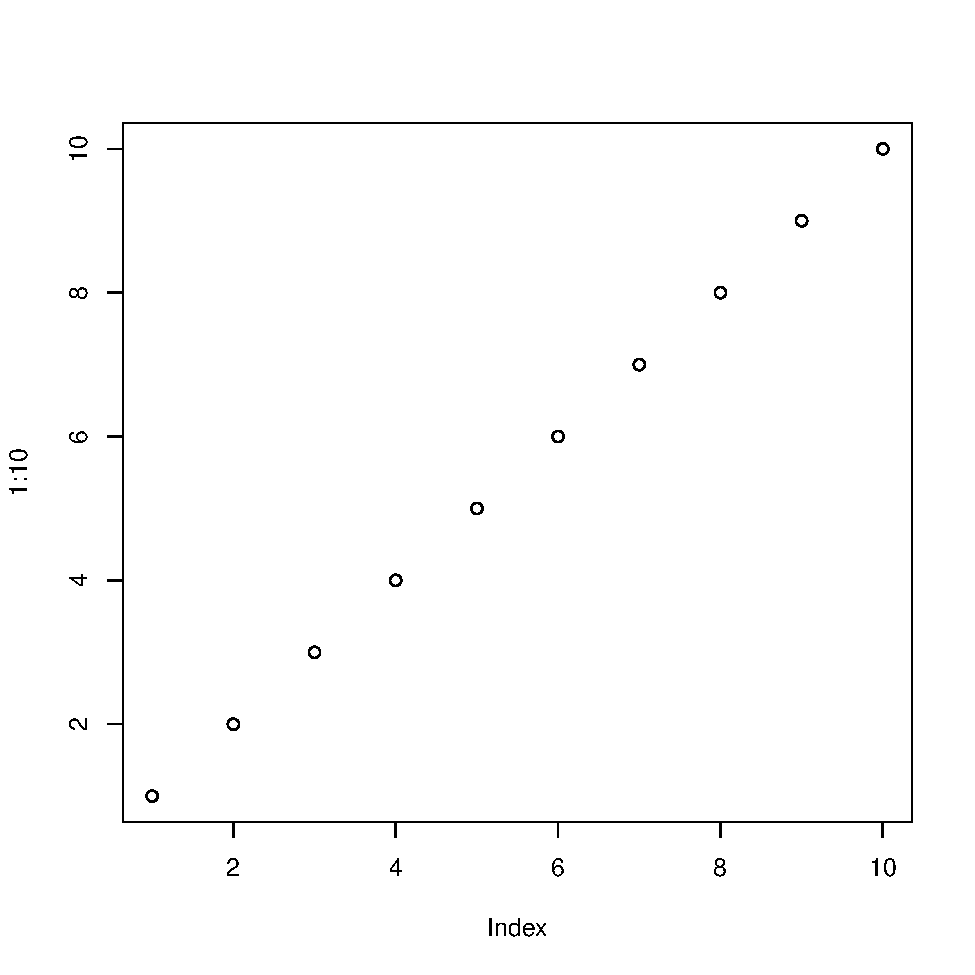
\includegraphics[width=6.5 in]{template_files/figure-pdf/apafg-myplot-1.pdf}


\figurenote{This is a note below the figure.}


\end{figure}

To refer to any figure or table, but the chunk label in curly braces.
For example, see Figure~\ref{apafg-myplot}. In
Figure~\ref{apafg-importedgraphic}, we import an image.

\begin{figure}[h!]
\caption{This is an imported graphic.}
\label{apafg-importedgraphic}

\includegraphics[width=0.85in]{orcid.png}


\figurenote{My note.}


\end{figure}

We can make a table the same way as a figure except that the label
prefix is \texttt{apatb-}. Again, this is different from the usual
quarto prefix \texttt{tbl-}, which will put the table table caption in
the wrong place and with non-APA formatting.

\begin{table}
\caption{Here is the table caption.}
\label{apatb-mytable}

\global\setlength{\Oldarrayrulewidth}{\arrayrulewidth}

\global\setlength{\Oldtabcolsep}{\tabcolsep}

\setlength{\tabcolsep}{0pt}

\renewcommand*{\arraystretch}{1.5}



\providecommand{\ascline}[3]{\noalign{\global\arrayrulewidth #1}\arrayrulecolor[HTML]{#2}\cline{#3}}

\begin{longtable*}[c]{|p{0.75in}|p{0.75in}}



\ascline{0.75pt}{000000}{1-2}

\multicolumn{1}{>{\centering}m{\dimexpr 0.75in+0\tabcolsep}}{\textcolor[HTML]{000000}{\fontsize{11}{11}\selectfont{Numbers}}} & \multicolumn{1}{>{\centering}m{\dimexpr 0.75in+0\tabcolsep}}{\textcolor[HTML]{000000}{\fontsize{11}{11}\selectfont{Letters}}} \\

\ascline{0.75pt}{000000}{1-2}\endhead



\multicolumn{1}{>{\centering}m{\dimexpr 0.75in+0\tabcolsep}}{\textcolor[HTML]{000000}{\fontsize{11}{11}\selectfont{1}}} & \multicolumn{1}{>{\centering}m{\dimexpr 0.75in+0\tabcolsep}}{\textcolor[HTML]{000000}{\fontsize{11}{11}\selectfont{A}}} \\





\multicolumn{1}{>{\centering}m{\dimexpr 0.75in+0\tabcolsep}}{\textcolor[HTML]{000000}{\fontsize{11}{11}\selectfont{2}}} & \multicolumn{1}{>{\centering}m{\dimexpr 0.75in+0\tabcolsep}}{\textcolor[HTML]{000000}{\fontsize{11}{11}\selectfont{B}}} \\





\multicolumn{1}{>{\centering}m{\dimexpr 0.75in+0\tabcolsep}}{\textcolor[HTML]{000000}{\fontsize{11}{11}\selectfont{3}}} & \multicolumn{1}{>{\centering}m{\dimexpr 0.75in+0\tabcolsep}}{\textcolor[HTML]{000000}{\fontsize{11}{11}\selectfont{C}}} \\





\multicolumn{1}{>{\centering}m{\dimexpr 0.75in+0\tabcolsep}}{\textcolor[HTML]{000000}{\fontsize{11}{11}\selectfont{4}}} & \multicolumn{1}{>{\centering}m{\dimexpr 0.75in+0\tabcolsep}}{\textcolor[HTML]{000000}{\fontsize{11}{11}\selectfont{D}}} \\

\ascline{0.75pt}{000000}{1-2}



\end{longtable*}



\arrayrulecolor[HTML]{000000}

\global\setlength{\arrayrulewidth}{\Oldarrayrulewidth}

\global\setlength{\tabcolsep}{\Oldtabcolsep}

\renewcommand*{\arraystretch}{1}

\tablenote{Here is the note below the table.}

\end{table}

To refer to this table in text, put the table's reference label in curly
braces like so: As seen in Table~\ref{apatb-mytable}, there is not much
information.

What if you want the tables and figures to be at the end of the
document? In the .pdf format, you can set the \texttt{floatsintext}
option to false. For .html and .docx documents, there is not yet an
automatic way to put tables and figures at the end. You can, of course,
just put them all at the end, in order. The reference labels will work
no matter where they are in the text.

\hypertarget{discussion}{%
\section{Discussion}\label{discussion}}

Describe results in non-statistical terms.

\hypertarget{limitations-and-future-directions}{%
\subsection{Limitations and Future
Directions}\label{limitations-and-future-directions}}

Every study has limitations. Based on this study, some additional steps
might include\ldots{}

\hypertarget{conclusion}{%
\subsection{Conclusion}\label{conclusion}}

Let's sum this up.

\hypertarget{references}{%
\section{References}\label{references}}

\hypertarget{refs}{}
\begin{CSLReferences}{1}{0}
\leavevmode\vadjust pre{\hypertarget{ref-CameronTrivedi2013}{}}%
Cameron, A. C., \& Trivedi, P. K. (2013). \emph{Regression analysis of
count data} (2nd ed.). Cambridge University Press.

\leavevmode\vadjust pre{\hypertarget{ref-cohen2003applied}{}}%
Cohen, J., Cohen, P., West, S. G., \& Aiken, L. S. (2003). \emph{Applied
multiple regression/correlation analysis for the behavioral sciences}.
Routledge.

\end{CSLReferences}

\newpage{}

\hypertarget{appendix}{%
\section{Appendix}\label{appendix}}

If there are multiple appendices, label them with level 1 headings as
Appendix A, Appendix B, and so forth.


\end{document}
